% =====================================================================
%  ijece-en.tex - Versi PADAT (maks ~14 halaman) dari ijece.tex.
%  Substansi, tabel, angka, gambar (16), dan 46 referensi dipertahankan;
%  yang dipangkas hanya verbositas narasi dan ukuran gambar.
% =====================================================================
\documentclass{iaesarticle}

\setlength{\headsep}{0.15in}
\usepackage{amsmath, amsfonts, amssymb, float, fancyhdr}
\usepackage[figuresright]{rotating}
\usepackage{authblk, graphicx, indentfirst, lastpage, lipsum}
\usepackage{pifont}
\renewcommand{\Authsep}{, }
\renewcommand{\Authand}{, }
\renewcommand{\Authands}{, }
\setlength{\affilsep}{0cm}
\renewcommand\Authfont{\normalsize}
\renewcommand\Affilfont{\fontsize{8}{10}\mdseries}
\makeatletter
\renewcommand{\@biblabel}[1]{[#1]\hfill}
\renewcommand\AB@authnote[1]{\textsuperscript{\normalfont\bfseries#1}}
\makeatother
\usepackage[font=normalsize]{subfig, caption}
\usepackage{epstopdf}
\usepackage[left=3cm, right=2.5cm, top=2.5cm, bottom=2.5cm, includehead, includefoot]{geometry}
\usepackage[justification=centering]{caption}
\captionsetup{labelsep=period}
\usepackage{titlesec}
\usepackage[table]{xcolor}
\titleformat{\section}
{\normalfont\normalsize\bfseries\uppercase}{\thesection}{1.7em}{}
\titleformat{\subsection}
{\normalfont\normalsize\bfseries}{\thesubsection}{.95em}{}
\titleformat{\subsubsection}
{\bfseries}{\thesubsubsection}{.2em}{}
\titlespacing*{\section}{0cm}{0.7cm}{0cm}
\usepackage{enumitem}
\usepackage[numbers,sort&compress]{natbib}
\usepackage{ragged2e}
\usepackage{hyperref,graphicx}
\usepackage{multirow}
\usepackage{tabularx}
\usepackage{booktabs}
\usepackage{fleqn}
\usepackage{tikz}
\usetikzlibrary{arrows.meta, positioning, shapes.geometric}

% Safe fallback for \orcidlink: if the IAES class/package already defines it,
% this line does nothing; otherwise it defines a no-op so the paper still compiles.
% In the official Overleaf template the ORCID icon is rendered by the class.
\providecommand{\orcidlink}[1]{}

\CopyrightLine[]{}{\textit{This is an open access article under the \textcolor{blue}{\underline{CC BY-SA}} license.}
\vspace{.5em}}

\author[1]{\bfseries Hero Yudo Martono}
\author[2]{\bfseries Nafisah Rahmadani Harahap}
\author[3]{\bfseries Iwan Syarif}
\author[4]{\bfseries Ferry Astika Saputra}
\affil[1,2,3,4]{Department of Informatics Engineering, Politeknik Elektronika Negeri Surabaya, Surabaya, Indonesia}

\title{Design of a cloud backup system based on multi-compression algorithms for ransomware attack mitigation}
\shorttitle{Design of a cloud backup system based on multi-compression algorithms ... (Martono)}

\begin{document}
\setcounter{page}{1}
\setlength{\parindent}{1.27cm}
\pagestyle{fancy}
\fancyhfoffset{0cm}

\journalname{International Journal of Electrical and Computer Engineering (IJECE)}
\journalshortname{Int J Elec \& Comp Eng}
\journalhomepage{http://ijece.iaescore.com}
\vol{99}
\no{1}
\months{Month}
\years{2099}
\issn{2088-8708}
\DOI{10.11591}
\pagefirst{1}
\pagelast{1x}
\IDpaper{42551}

\maketitle

\hrule
\vspace{.1em}
\hrule
\vspace{.5em}
\noindent
\parbox[t][][s]{0.315\textwidth}{%
\textbf{Article Info}
\vspace{.5em}
\hrule
\vspace{.5em}
\begin{history}
\vspace{.5em}
Received month dd, yyyy

Revised month dd, yyyy

Accepted month dd, yyyy

\vspace{.7em}
\end{history}
\vspace{.5em}
\hrule
\vspace{.5em}
\begin{keyword}
\vspace{.5em}
Air-gapped backup \sep
Anomaly detection \sep
Cloud backup and restore \sep
Lossless compression \sep
Ransomware resilience
\vspace{.5em}
\end{keyword}
\vspace{\fill}
}
\parbox{0.020\textwidth}{\hspace{0.5em}}
\parbox[t][][s]{0.65\textwidth}{%
\begin{abstract}
\vspace{.3em}
Ransomware threatens the availability and integrity of data in cloud storage, and conventional backups remained vulnerable when the repository was directly reachable from the primary system, while single-algorithm compression was inefficient for heterogeneous file types. This study proposed a cloud backup system that integrated a logical air-gapped mechanism with adaptive multi-algorithm lossless compression to improve resilience and storage efficiency. The system used SHA-256 hash verification, metadata analysis, and file-structure inspection to distinguish legitimate backup encryption from ransomware-induced modification. Evaluation was performed in a controlled manner using a simulated attack model, without executing real malware, on a limited synthetic dataset of 43 files of varying types and sizes, under both normal and attacked conditions, and replicated on AWS EC2 (Windows and Linux). For low-entropy text files, compression reduced storage by up to 89.5\% (logs) and 81.1\% (CSV), whereas already-compressed files (JPG, XLSX) approached 0\%, consistent with information theory. The adaptive strategy completed the whole dataset about $21\times$ faster than static Gzip while still saving 43.3\% of storage. The system recovered all 43 affected files without error and, under the controlled conditions, achieved 0\% false positive rate (FPR) and 0\% false negative rate (FNR). Overall, the proposed approach strengthened the security, resilience, and storage efficiency of cloud backup against ransomware.
\end{abstract}
}
\parbox[l]{\textwidth}{%
\rule{0.275\textwidth}{0.5pt} \hspace{0.5cm} \hrulefill
\\
\emph{\textbf{Corresponding Author:}}
\vspace{.5em}\\
Hero Yudo Martono\\
Department of Informatics Engineering, Politeknik Elektronika Negeri Surabaya\\
Surabaya, Indonesia\\
Email: hero@pens.ac.id
}
\vspace{.5em}
\hrule
\vspace{.1em}
\hrule

\section{Introduction}
\label{sec:introduction}
Over the past decade, digital transformation---particularly in finance---has driven an exponential growth of data (transaction records, logs, user data, financial reports, and audit documents) that must be archived securely and efficiently for operational, audit, and regulatory purposes \cite{1}, \cite{2}. A single financial institution may generate hundreds of gigabytes to terabytes daily, demanding storage that is secure, economical, and backed by mechanisms that keep data available and intact.

Among cyber threats, ransomware is the most alarming: it encrypts victims' data and demands a ransom, and modern variants also target network-connected backup infrastructure \cite{6}, \cite{7}, \cite{8}. Once backups are infected, recovery becomes impossible, causing operational, financial, and reputational damage \cite{9}; Sophos reports that about 43\% of devices in financial organizations were affected in 2024. Conventional always-connected backups are therefore inadequate. A proven countermeasure is the air-gapped architecture, which isolates backup storage---physically or logically---from the primary network \cite{10}. Because a fully physical air-gap is costly and complex for small and medium organizations, this study adopts a logical air-gap using controlled mounting and isolated media, prioritizing affordability, ease of deployment, and compatibility with common cloud infrastructures.

The scale of the threat has surged: a survey of 50+ articles (2020--2025) records global losses exceeding USD~30 billion in 2023 ($\approx$900\% rise from 2015), 493 million attacks in 2022, an average ransom of USD~2.73 million in 2024, and 21 days average disruption \cite{41}. Ransomware has entered the \textit{data-exfiltration} era with \textit{double}/\textit{triple extortion} and a \textit{Ransomware-as-a-Service} (RaaS) model, while academic research lags behind real attack patterns \cite{23}, \cite{26}. Preventing infection alone is no longer sufficient \cite{42}, \cite{46}. The literature organizes defenses via the \textit{Detection--Avoidance--Mitigation} (DAM) framework \cite{42}; within it, this study occupies the mitigation and recovery stage, ensuring data remain recoverable even when early detection fails, rather than competing on \textit{machine-learning} detection accuracy.

Storage efficiency is equally important. For rarely accessed data, organizations use cold cloud storage, where lossless compression trims cost without harming integrity \cite{13}. However, prior work generally treats backup security, ransomware mitigation, or compression separately \cite{14}, and mostly relies on a single static algorithm despite the non-uniform compression behavior of different file types.

The link between compression and security stems from \textit{entropy}. Shannon's theory sets the lossless limit as $H(X) = -\sum_{i} p(x_i)\log_2 p(x_i)$: low-entropy files (CSV, logs) are highly redundant and compress well, whereas high-entropy files (encrypted or already-compressed JPG) are near-random and barely compress. Two consequences follow: (i) the algorithm should adapt to file entropy/type, and (ii) a sudden entropy spike can signal illegitimate encryption---though \textit{Format-Preserving Encryption} (FPE) can evade entropy-based detection by preserving structure. This defines our \textit{research gap}: no single framework yet unites (a) adaptive compression by file characteristics, (b) ransomware-resilient backup isolation, and (c) integrity verification based on hash and metadata rather than entropy alone.

Accordingly, this study proposes an integrated cloud backup system combining an air-gapped architecture with an adaptive framework that dynamically selects among five lossless algorithms (Gzip, Zstandard, Brotli, LZ4, Snappy) via rule-based selection on file size and type. It further embeds multi-indicator anomaly detection---SHA-256 hash analysis, metadata validation, and file-structure inspection---to separate ransomware encryption from legitimate AES-256 encryption. The contribution is thus an integrated approach that simultaneously addresses ransomware resilience, backup isolation, adaptive compression efficiency, and integrity verification within one framework for cloud-based financial data infrastructures \cite{19}, \cite{20}.

We therefore hypothesize that an entropy-aware adaptive selection does not maximize any single objective in isolation but instead trades a small, bounded loss in storage saving for a disproportionately large reduction in execution time, while keeping recovery latency low and approximately linear in data volume. Concretely, we expect the adaptive strategy to retain most of the storage saving achievable by a slow high-ratio algorithm (within single-digit percentage points), yet complete compression about an order of magnitude faster, and to recover all affected files with a recovery time that scales predictably with dataset size rather than with the type of attack. This explicit trade-off among storage savings, execution time, and recovery latency is the central claim evaluated in Section~\ref{sec:results}.

\section{Related Work}
\label{sec:related_work}
Prior studies on cloud backup, compression, and ransomware mitigation mostly address a single aspect in isolation and rarely contrast air-gapped with conventional connected backups. Table~\ref{tab:related_work} compares representative studies with the proposed system.

\begin{table}[htbp]
\centering
\fontsize{8pt}{10pt}\selectfont
\caption{Related work}
\label{tab:related_work}
\begin{tabularx}{\textwidth}{@{}c p{2.2cm} X X X X@{}}
\hline
\textbf{No} & \textbf{Study} & \textbf{Research Focus} & \textbf{Methods} & \textbf{Limitations} & \textbf{Contribution of this study} \\
\hline
1 & Mazel \textit{et al.}, 2024 & Compression algorithm evaluation & Zstandard, zlib, LZ4 & No backup security & Integrates compression with backup \\
2 & Jaranilla and Choi, 2023 & Compression trade-offs in key--value stores & Gzip, Zstd, LZ4, Snappy & Storage-engine focus only & Applied within backup for storage efficiency \\
3 & Shynu \textit{et al.}, 2020 & Secure data reduction for cloud-edge & Deduplication + encryption & No ransomware recovery & Cloud backup with anomaly detection and recovery \\
4 & Novak \textit{et al.}, 2024 & Malware detection for backup systems & Multistage detection & No multi-algorithm compression & Evaluates multiple algorithms with recovery \\
5 & Sahu and Panda, 2025 & Compression study & Snappy, Gzip, BZIP2 & Limited efficiency analysis & Integrates efficiency and security \\
6 & NIST (2024) guideline & Secure offline backup & Physical/logical air-gapped & No storage optimization/compression & Combines air-gap + adaptive compression + detection \\
\hline
\end{tabularx}
\end{table}

Mazel \textit{et al.}~\cite{36} and Jaranilla and Choi~\cite{37} evaluated lossless compression algorithms and their trade-offs without any backup-security or ransomware context; Shynu \textit{et al.}~\cite{38} reduced cloud storage through secure deduplication but did not address ransomware recovery; and Novak \textit{et al.}~\cite{29} proposed malware detection for backup systems without comprehensively optimizing storage. The novelty here is integrating air-gapped protection, adaptive multi-algorithm lossless compression, and hash/metadata anomaly detection in one architecture, improving resilience, efficiency, automated recovery, and practical deployment.

To position this work against the ransomware-detection mainstream: classical ML achieves high accuracy with feature selection \cite{31}, deep models (CNN, LSTM, CNN--LSTM) reach 96--99\% on balanced datasets \cite{30}, and real-time AES-NI monitoring can halt attacks after 10--15 files \cite{32}. Yet these face outdated datasets, cross-platform difficulty, and evasion such as FPE \cite{43}, fileless, and Living-off-the-Land. This study does not compete on detection accuracy; it strengthens the \textit{mitigation/recovery} layer, aligned with backup-strategy work (3-2-1, immutable/WORM, air-gapped) reporting high recovery without ransom \cite{44} and structured incident response \cite{45}. It is therefore complementary to ML detectors: when detection fails, integrity checks and isolated recovery guarantee availability.

Conceptually, an air-gapped backup differs from a conventional connected backup on every axis that matters for ransomware resilience: the repository is isolated (physically or logically) rather than reachable from the primary system, so the risk of backup infection is minimal rather than potentially compromised, data integrity and recovery remain reliable rather than uncertain, and--combined with adaptive multi-algorithm compression--storage efficiency reaches up to 70--80\% rather than the moderate savings of a single static codec. In practice, many small and medium organizations still rely on connected cloud backups with single-algorithm compression, which remain vulnerable because repositories are directly reachable from compromised systems. The proposed system adds logical air-gapped isolation, automated integrity verification, adaptive compression, and ransomware-aware recovery, achieving up to 70--80\% storage reduction for large structured data while maintaining 100\% recovery in simulation.

\section{Method}
\label{sec:method}
This study uses a quantitative experimental design to evaluate a cloud backup system integrating multiple lossless compression algorithms \cite{22}. Each algorithm is tested independently, evaluating storage efficiency, processing time, and resilience to simulated ransomware. The system adopts a hybrid air-gapped architecture combining offline local and cloud storage \cite{21}, \cite{27}, in an environment resembling real financial information systems \cite{29}.

\subsection{System architecture}
The architecture has three logical layers. The \emph{application layer} manages upload, backup, and restore; each file undergoes SHA-256 hash computation, metadata extraction, and structure analysis to form an integrity baseline distinguishing legitimate modification from malicious alteration. The \emph{protection and compression layer} inspects metadata, then compresses first using one of five algorithms and only then encrypts with AES-256. This compress-then-encrypt order is essential: encrypted data has high entropy and cannot be compressed effectively, so compressing plaintext first yields genuine savings before confidentiality is applied \cite{9}. The \emph{storage and detection layer} stores encrypted-compressed files in an air-gapped environment and synchronizes to cloud storage (Google Drive API or Amazon S3) for redundancy; on detecting ransomware, it auto-recovers from air-gapped storage via decryption and decompression. Figure~\ref{fig:architecture} shows the flow.

\begin{figure}[htbp]
\centering
\resizebox{0.9\textwidth}{!}{%
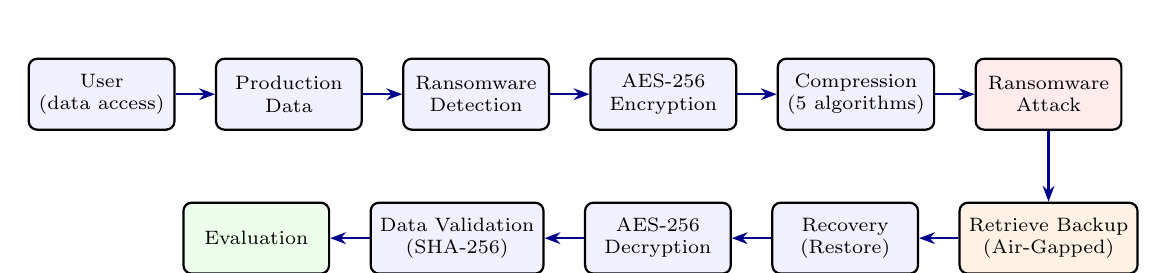
\begin{tikzpicture}[
    font=\scriptsize,
    node distance=0.4cm and 0.5cm,
    stage/.style={draw, rounded corners=3pt, minimum width=1.85cm, minimum height=0.9cm,
                  align=center, fill=blue!6, thick},
    ar/.style={-{Stealth[length=2mm]}, thick, blue!55!black}
]
\node[stage] (user)  {User\\(data access)};
\node[stage, right=of user] (prod)  {Production\\Data};
\node[stage, right=of prod] (det)   {Ransomware\\Detection};
\node[stage, right=of det]  (enc)   {AES-256\\Encryption};
\node[stage, right=of enc]  (comp)  {Compression\\(5 algorithms)};
\node[stage, right=of comp, fill=red!8] (atk) {Ransomware\\Attack};
\foreach \a/\b in {user/prod, prod/det, det/enc, enc/comp, comp/atk}
   \draw[ar] (\a) -- (\b);
\node[stage, below=0.9cm of atk, fill=orange!10] (bkp) {Retrieve Backup\\(Air-Gapped)};
\draw[ar] (atk) -- (bkp);
\node[stage, left=of bkp]  (rest) {Recovery\\(Restore)};
\node[stage, left=of rest] (dec)  {AES-256\\Decryption};
\node[stage, left=of dec]  (val)  {Data Validation\\(SHA-256)};
\node[stage, left=of val, fill=green!8]  (eval) {Evaluation};
\foreach \a/\b in {bkp/rest, rest/dec, dec/val, val/eval}
   \draw[ar] (\a) -- (\b);
\end{tikzpicture}%
}
\vspace{.5em}
\caption{Proposed system architecture integrating AES-256 encryption, multi-algorithm compression, and air-gapped backup for ransomware protection}
\label{fig:architecture}
\end{figure}

\subsection{Dataset and data acquisition}
The dataset is synthetically generated to resemble enterprise/financial backup structures adapted from PT Equnix; no real production data were used, for privacy compliance \cite{27}. Table~\ref{tab:dataset} summarizes its 43 files.

\begin{table}[htbp]
\centering
\fontsize{8pt}{10pt}\selectfont
\caption{Characteristics of the dataset used in the experiments}
\label{tab:dataset}
\begin{tabularx}{\textwidth}{@{}c p{1.9cm} p{1.3cm} c p{1.9cm} X@{}}
\hline
\textbf{No} & \textbf{Data Type} & \textbf{Format} & \textbf{Files} & \textbf{Size Range} & \textbf{Description} \\
\hline
1 & Structured transaction data & CSV & 9 & 500 KB -- 1 GB & Structured text with repetitive patterns; sizes varied to analyze ratio and time. \\
2 & System log data & TXT/LOG & 9 & 500 KB -- 1 GB & Application logs/audit trails; common ransomware targets. \\
3 & Visual documents & JPG & 14 & 154 -- 249 KB & Binary already-compressed files; test lossless limits. \\
4 & Spreadsheet documents & XLSX & 11 & 500 KB -- 650 MB & Operational and financial reports. \\
\hline
\multicolumn{3}{@{}l}{\textbf{Total}} & \textbf{43 files} & & \\
\hline
\end{tabularx}
\end{table}

A synthetic dataset was chosen deliberately: existing public ransomware datasets target malware classification, not backup-recovery of victim documents; real production financial data cannot be used for privacy reasons; and synthetic data give full control over file types, sizes, and content for reproducible testing. The authors acknowledge that a 43-file synthetic set limits generalizability---discussed in the conclusion, with the \textit{Silesia Compression Corpus} suggested for further validation.

\subsection{AES-256 encryption and decryption}
The system uses AES-256 symmetric encryption. In backup, the plaintext is compressed first, and the compressed output is encrypted, producing ciphertext stored in air-gapped and cloud storage; in restore, the file is decrypted then decompressed, and integrity is verified with SHA-256. Figure~\ref{fig:aes} illustrates the symmetric-key process.

\begin{figure}[htbp]
\centering
\resizebox{0.78\textwidth}{!}{%
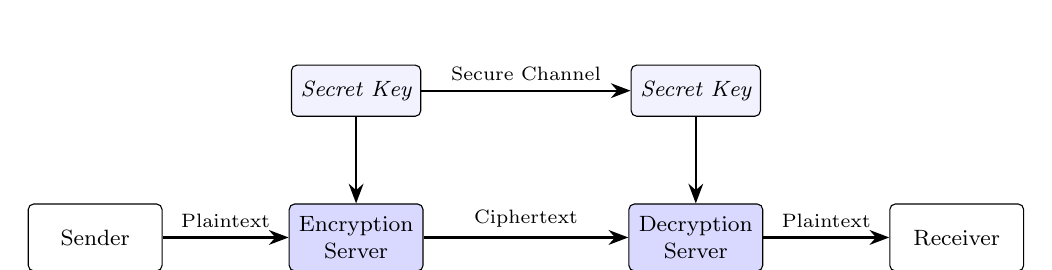
\begin{tikzpicture}[
    node distance=1.2cm and 1.6cm,
    box/.style={draw, rounded corners=2pt, minimum width=1.7cm, minimum height=0.85cm, align=center, font=\footnotesize},
    keyb/.style={draw, rounded corners=2pt, minimum width=1.5cm, minimum height=0.65cm, align=center, font=\footnotesize\itshape, fill=blue!5},
    ar/.style={-{Stealth[length=2.5mm]}, thick},
    font=\footnotesize
]
\node[box] (sender) {Sender};
\node[box, right=of sender, fill=blue!15] (enc) {Encryption\\Server};
\node[box, right=2.6cm of enc, fill=blue!15] (dec) {Decryption\\Server};
\node[box, right=of dec] (recv) {Receiver};
\node[keyb, above=1.1cm of enc] (k1) {Secret Key};
\node[keyb, above=1.1cm of dec] (k2) {Secret Key};
\draw[ar] (sender) -- node[above]{\scriptsize Plaintext} (enc);
\draw[ar, line width=1pt] (enc) -- node[above]{\scriptsize Ciphertext} (dec);
\draw[ar] (dec) -- node[above]{\scriptsize Plaintext} (recv);
\draw[ar] (k1) -- node[above, font=\scriptsize]{Secure Channel} (k2);
\draw[ar] (k1) -- (enc);
\draw[ar] (k2) -- (dec);
\end{tikzpicture}%
}
\vspace{.5em}
\caption{AES-256 encryption and decryption process using a symmetric secret key}
\label{fig:aes}
\end{figure}

\subsection{Compression algorithm implementation}
Compression uses a rule-based selection (\textit{rule-based decision tree}) rather than machine learning, chosen for low overhead, lightweight implementation, and fast, predictable decisions suited to low-latency backup. The algorithm is selected by file type and size (Table~\ref{tab:rule_selection}): small-to-medium text (CSV/LOG/TXT $\leq 100$~MB) to Snappy/LZ4 for speed; large text to Zstandard for ratio; already-compressed JPG to lightweight algorithms; XLSX to LZ4/Zstandard by size. A priority order with fallback (Gzip as final safety net) guarantees every file is backed up. Five open-source algorithms are implemented in Python and applied identically to each file, measuring compression ratio and processing time \cite{36}, \cite{37}, \cite{38}, \cite{39}, \cite{22}.

\begin{table}[htbp]
\centering
\fontsize{8pt}{10pt}\selectfont
\caption{Compression algorithm selection rules by file type and size (priority order with fallback)}
\label{tab:rule_selection}
\begin{tabular}{l l l}
\hline
\textbf{File type} & \textbf{Size condition} & \textbf{Algorithm priority order} \\
\hline
CSV / LOG / TXT & $\leq 100$ MB & Snappy $\rightarrow$ LZ4 $\rightarrow$ Zstandard \\
CSV / LOG / TXT & $> 100$ MB & Zstandard $\rightarrow$ Gzip \\
JPG & all sizes & Snappy $\rightarrow$ LZ4 $\rightarrow$ Gzip \\
XLSX & $\leq 250$ MB & LZ4 $\rightarrow$ Zstandard \\
XLSX & $> 250$ MB & Zstandard $\rightarrow$ Gzip \\
Others & all sizes & Gzip (fallback) \\
\hline
\end{tabular}
\end{table}

\subsection{Backup and recovery procedure}
Backup begins with SHA-256 baseline computation, then compression, then AES-256 encryption of the compressed output (compress-then-encrypt); files are staged air-gapped and mirrored to cloud. Under normal conditions (no anomaly), the system stops after backup, avoiding unnecessary recovery overhead. Recovery is triggered only on anomalies (hash mismatch, metadata inconsistency, unauthorized encryption): data are retrieved from air-gapped storage, decrypted then decompressed, and validated against the baseline hash. The overall flow (start $\rightarrow$ upload $\rightarrow$ hash $\rightarrow$ encrypt $\rightarrow$ compress $\rightarrow$ air-gapped backup; and, on attack, retrieve backup $\rightarrow$ restore $\rightarrow$ decrypt $\rightarrow$ decompress $\rightarrow$ validate) follows the architecture of Figure~\ref{fig:architecture}.

\subsection{Ransomware attack simulation and detection}
Resilience was evaluated by simulating ransomware without executing real malware, based on three real vulnerability patterns: CVE-2017-0144 (encrypt-and-hold), CVE-2021-36934 (overwrite/corruption), and CVE-2018-8453 (metadata/header corruption). Detection combines SHA-256 hash verification, metadata analysis (size, modification time, type, extension), and air-gapped backup validation: each file's baseline hash is re-verified during inspection, and any discrepancy between the primary and air-gapped copies classifies the file as normal, legitimately modified, or a ransomware indication.

\subsection{Performance evaluation metrics}
Storage efficiency is reported as the Storage Saving, i.e., the percentage reduction in size after compression (one minus the compressed-to-original size ratio). A combined efficiency score balances storage saving and speed with equal weight (0.5 each), normalized to a 0--100 scale and interpreted as excellent ($\geq$90), good (80--89), fair (70--79), or poor ($<$70). Recovery speed is reported as the Recovery Time Objective (RTO), the elapsed time from anomaly detection to full restoration. Detection reliability is reported as the false positive rate (FPR) and false negative rate (FNR) in percent, where lower values indicate higher reliability.

\subsection{Experimental setup and reproducibility}
\label{sec:repro}
To ensure the simulation and measurements are reproducible, we fix the implementation, parameters, and procedure as follows. The system is implemented in Python and evaluated on two environments summarized in Table~\ref{tab:experimental_setup}: a local Windows~11 machine (the initial development environment) and a cloud replication on AWS~EC2 with Windows Server~2022 and Ubuntu~22.04 (the primary measurement/validation environment). All reported quantitative figures (compression ratio, throughput, RTO, and repeated-trial statistics) come from controlled EC2 measurements; testing on two platforms verifies cross-platform consistency and mitigates the single-platform generalizability limitation.

\begin{table}[htbp]
\centering
\fontsize{8pt}{10pt}\selectfont
\caption{Experimental setup across two test environments}
\label{tab:experimental_setup}
\begin{tabularx}{\textwidth}{@{}l X X@{}}
\hline
\textbf{Component} & \textbf{Local (Windows)} & \textbf{Cloud (AWS EC2)} \\
\hline
Operating System & Windows 11 (64-bit) & Windows Server 2022 \& Ubuntu 22.04 \\
CPU & Intel Core i7-11800H (8-core) & t3.xlarge (4 vCPU) / t3.large (2 vCPU) \\
RAM & 16 GB & 16 GB (Windows) / 8 GB (Linux) \\
Language & Python 3.10 & Python 3.11 / 3.10 \\
Compression & \multicolumn{2}{l}{Gzip, Zstandard, Brotli, LZ4, Snappy} \\
Cryptography & \multicolumn{2}{l}{PyCryptodome (AES-256), hashlib (SHA-256)} \\
Air-gapped media & External SSD / VHDX & Separate EBS volume (D: / \texttt{/mnt/airgap}) \\
Cloud Storage & Google Drive API & Amazon S3 \\
\hline
\end{tabularx}
\end{table}

Cryptography uses the PyCryptodome library: AES-256 in a symmetric key configuration with a 256-bit key, and SHA-256 via Python's \texttt{hashlib} for the integrity baseline. Compression uses five open-source libraries with fixed, default-to-balanced settings applied uniformly to every file: Gzip (level~6), Zstandard (level~3), Brotli (quality~11 for ratio-oriented runs), LZ4 (fast mode), and Snappy (default). The rule-based selector (Table~\ref{tab:rule_selection}) is deterministic: given the same file type and size, it always chooses the same algorithm, so no randomness enters the pipeline. The compress-then-encrypt order is always enforced.

Measurement procedure: processing time is taken as wall-clock time around the compression call; throughput is dataset size divided by that time; CPU and RAM utilization are sampled with \texttt{psutil}; and Shannon entropy is computed per byte over the full file. To account for run-to-run variation, each compression measurement on the full dataset ($\approx$531~MB, 43 files) is repeated five times, and we report the mean and standard deviation. Recovery time (RTO) is measured as the wall-clock interval from anomaly detection to the completion of restoring and validating all 43 files from air-gapped storage. The synthetic dataset generation (file types, sizes, and counts of Table~\ref{tab:dataset}) and the three controlled attack patterns (CVE-2017-0144, CVE-2018-8453, CVE-2021-36934) are scripted so that the entire backup--attack--recovery cycle can be regenerated end-to-end.

\section{Results and Discussion}
\label{sec:results}
The proposed system delivered reliable protection, compression, and recovery: all files kept identical SHA-256 hash values (zero alteration), Zstandard/Brotli gave the highest compression while Snappy/LZ4 were fastest, and the air-gapped mechanism enabled 100\% recovery with zero errors under simulation.

\subsection{Normal conditions (no attack)}
The main workflow was verified end-to-end. The system establishes a secure cloud connection via token/role-based authentication (OAuth~2.0 for Google Drive; IAM role for S3), generating a unique session ID per backup, then uploads and validates files with SHA-256 hashing and metadata before compression/encryption.

Integrity validation computes a unique SHA-256 hash per file as a digital fingerprint, stored together with metadata (size, timestamp, MIME type, extension, structure) as a JSON baseline. For each file the validation recomputes the hash and metadata and flags an anomaly whenever either deviates from the baseline, otherwise marking the file as safe. This combination detects content-level and structural changes (altered timestamps, suspicious extensions, corrupted headers); in the normal run all files were verified as safe (\texttt{detected\_ransom\_files: []}) before compression/encryption.

The system then applies AES-256 to each validated file (using the loaded encryption key), writing a \texttt{.enc} output and logging the encryption status. Encryption runs only after successful hash/metadata validation, so legitimate backup encryption (authorized keys, verified files) is cleanly distinguished from ransomware behavior.

\subsection{Compression performance by algorithm}
Table~\ref{tab:compression_results} reports the average storage saving (SS) at the plaintext stage for each file type and algorithm.

\begin{table}[htbp]
\centering
\fontsize{8pt}{10pt}\selectfont
\caption{Average storage saving (\%) by file type and algorithm (43 files)}
\label{tab:compression_results}
\begin{tabular}{l c c c c c}
\hline
\textbf{File Type} & \textbf{Gzip} & \textbf{Zstandard} & \textbf{Brotli} & \textbf{LZ4} & \textbf{Snappy} \\
\hline
Log/TXT & 88.5 & 87.6 & \textbf{89.5} & 77.4 & 80.2 \\
CSV     & 79.9 & 78.7 & \textbf{81.1} & 66.6 & 66.4 \\
XLSX    & 1.1  & 0.0  & 0.0  & 0.0  & 0.0  \\
JPG     & 0.1  & 0.0  & 0.0  & 0.0  & 0.0  \\
\hline
\end{tabular}
\end{table}

Low-entropy text yields the highest savings (Log/TXT up to 89.5\%, CSV up to 81.1\% with Brotli; Gzip/Zstandard follow closely above 78\%). Fast algorithms (LZ4/Snappy) give slightly lower savings (66--80\%) at far shorter times---ideal for real-time scenarios. JPG and XLSX (already compressed) approach 0\%, confirming the lossless limit on high-entropy data and validating the rule-based adaptive selection (Figure~\ref{fig:overall_analysis}).

\begin{figure}[htbp]
\centering
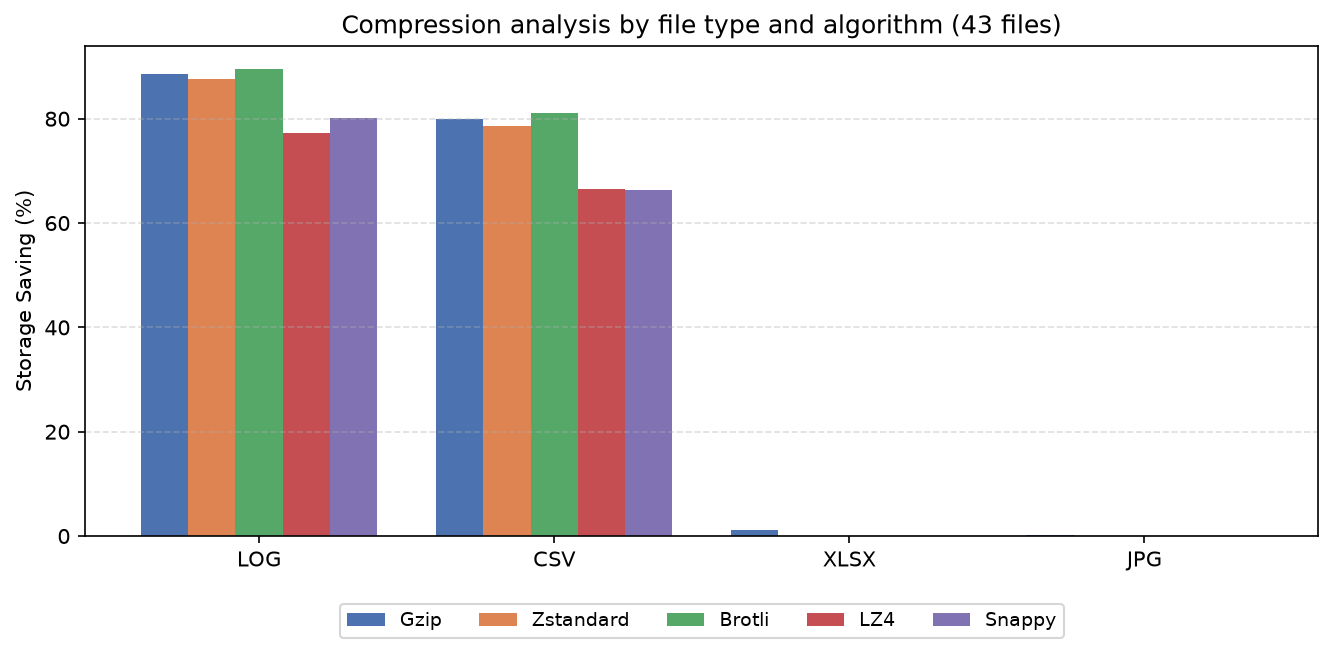
\includegraphics[width=0.62\textwidth]{figures/figure10_compression_en.png}
\vspace{.4em}
\caption{Overall analysis results of the algorithms}
\label{fig:overall_analysis}
\end{figure}

Compression was then repeated five times on the full dataset (43 files, $\approx531$~MB) on AWS EC2 (Ubuntu 22.04). Table~\ref{tab:comp_stats} reports mean$\pm$std of time, throughput, and CPU/RAM (via \texttt{psutil}).

\begin{table}[htbp]
\centering
\fontsize{8pt}{10pt}\selectfont
\caption{Statistical analysis of compression performance (5 trials, 43 files $\approx$531 MB)}
\label{tab:comp_stats}
\begin{tabular}{l c c c c c}
\hline
\textbf{Algorithm} & \textbf{Mean time (s)} & \textbf{Std (s)} & \textbf{Throughput (MB/s)} & \textbf{CPU (\%)} & \textbf{RAM (MB)} \\
\hline
Gzip      & 17.427 & 0.062 & 30.5  & 100.0 & 6.3 \\
Brotli    & 10.468 & 0.237 & 50.7  & 100.0 & 5.1 \\
Zstandard & 1.721  & 0.016 & 308.7 & 99.9  & 3.4 \\
LZ4       & 0.896  & 0.011 & 592.7 & 100.0 & $<$1 \\
Snappy    & 0.831  & 0.003 & 639.0 & 99.3  & 0.9 \\
\hline
\end{tabular}
\end{table}

The very small std (e.g., Snappy 0.003~s, Zstandard 0.016~s) shows stable, consistent performance. Throughput spans a wide range (Snappy/LZ4 $>590$~MB/s, $\approx20\times$ Gzip's 30.5~MB/s), while Zstandard balances speed (308.7~MB/s) with a high ratio. Near-100\% CPU confirms the process is CPU-bound; small RAM ($<7$~MB) keeps it lightweight for constrained environments---an objective basis for adaptive selection.

\subsection{Comparison against baselines}
The adaptive strategy was compared to (i) no compression, (ii) static Gzip, and (iii) static Zstandard on the full dataset (Table~\ref{tab:baseline_comparison}).

\begin{table}[htbp]
\centering
\fontsize{8pt}{10pt}\selectfont
\caption{Comparison of the adaptive strategy against baselines (43 files, $\approx$531 MB)}
\label{tab:baseline_comparison}
\begin{tabular}{l c c c c}
\hline
\textbf{Strategy} & \textbf{Final Size (MB)} & \textbf{Saving (\%)} & \textbf{Time (s)} & \textbf{Throughput (MB/s)} \\
\hline
No compression        & 531.2 & 0.00  & --    & -- \\
Static-Gzip           & 265.1 & 50.09 & 18.84 & 28.2 \\
Static-Zstandard      & 271.1 & 48.96 & 1.94  & 273.8 \\
\textbf{Adaptive (proposed)} & 301.3 & 43.28 & \textbf{0.87} & \textbf{611.8} \\
\hline
\end{tabular}
\end{table}

Static Gzip achieves the highest saving (50.1\%) but is slow (18.84~s; 28.2~MB/s). The adaptive strategy prioritizes speed---finishing in 0.87~s, $\approx21\times$ faster than static Gzip and $2.2\times$ faster than static Zstandard---while still saving 43.3\%. Trading 6.8 percentage points of saving for a dramatic throughput gain (611.8 vs 28.2~MB/s) is advantageous for low-RTO, resource-constrained backup. The adaptive mechanism's key benefit is thus the optimal balance between storage efficiency and speed.

\subsection{Entropy analysis}
Shannon entropy $H(X)$ (bits/byte, 0--8) per file type relates both to storage saving and to attack detection (Table~\ref{tab:entropy}).

\begin{table}[htbp]
\centering
\fontsize{8pt}{10pt}\selectfont
\caption{Shannon entropy per file type: relation to storage saving, and change before/after a ransomware encryption attack}
\label{tab:entropy}
\begin{tabular}{l c c c c}
\hline
\textbf{File Type} & \textbf{Entropy (bits/byte)} & \textbf{Saving (\%)} & \textbf{After attack} & \textbf{$\Delta H$} \\
\hline
CSV  & 4.573 & 66.4 & 8.000 & $+3.453$ \\
LOG  & 5.232 & 80.0 & 8.000 & $+2.777$ \\
XLSX & 7.962 & $\approx$0 & 8.000 & $+0.036$ \\
JPG  & 7.940 & $\approx$0 & 8.000 & $+0.060$ \\
\hline
\end{tabular}
\end{table}

Text files (CSV, LOG) have low entropy (4.6--5.2) and compress by 66--80\%, while JPG/XLSX near the 8.0 limit barely compress---a strong inverse correlation justifying file-type-based selection. After an encrypt-and-hold attack, low-entropy files spike to 8.0 ($\Delta H$ up to $+3.45$), a clear sign of unauthorized encryption; already-high-entropy files change little, exposing the weakness of entropy-only detection (e.g., FPE) and reinforcing our reliance on hash/metadata integrity, which detects \textit{any} change regardless of entropy.

\subsection{Recovery time scalability}
The backup--recovery cycle was measured from 50~MB to 1~GB, recovering all files at every size. Both backup and recovery time grow approximately linearly with volume: recovery rises from 0.344~s at 51.2~MB, through 1.797~s at 250.9~MB and 4.020~s at 500.5~MB, to 7.731~s at 1001.0~MB (backup time from 0.187~s to 5.927~s over the same range). The fitted recovery rate is $\approx0.0073$~s/MB (std only 0.0005), confirming the deterministic workflow (SHA-256, AES-256 decryption, decompression). Even a 1~GB dataset recovers fully in $\approx7.7$~s with integrity preserved, enabling reliable RTO projection for enterprise scale.

\subsection{Air-gapped backup storage implementation and structure}
As an added protection layer, the system implements a logical (online) air-gap on a separate medium (external SSD/VHDX) that is not permanently accessible: it is mounted only during a backup or restore session, minimizing unauthorized access and network-borne malware propagation. The medium stays within the system environment but is reachable only under system-defined conditions (access control, active sessions, limited mounting) with no active network connection during storage. This is not as strong as a fully offline physical air-gap---advanced memory-resident malware could attempt access while the medium is mounted---but the residual risk is mitigated by short mount durations, automatic disconnection after backup, SHA-256/metadata verification, isolated repositories, and restricted sessions, offering a practical, cost-effective option for small and medium organizations. On the isolated medium, backups are organized by compression algorithm alongside a JSON hash-storage file holding SHA-256 values of the original and backup files for integrity validation.

Transfers to air-gapped storage are controlled and logged automatically, recording the reset/mounting stages and the subsequent short data transfer (destination, processing time, and success status); this logging enables detailed audit and trace of backup activity, evidencing that transfers are performed separately rather than continuously. Monitoring uses an interactive dashboard summarizing file status, compression ratio, compression time, validation results, and restore status per algorithm in real time. During the normal simulation the system detected no anomalies in structure or metadata (size, format/extension, last-modified timestamp), and matching SHA-256 hashes confirmed no content change or corruption during backup.

\subsection{Simulation under disrupted conditions (ransomware attack)}
Under disrupted conditions, main-system files were corrupted by simulated attacks while backups remained secure in isolated air-gapped storage; on detecting hash/metadata anomalies the system automatically referred to backup copies for recovery.

Three damage types were tested on the small-to-medium target file \texttt{finance\_log\_500KB.log}, each with a distinct impact. Encrypt-and-hold (CVE-2017-0144) applies a controlled WannaCry-style content modification: the file fully changes (size and timestamp altered, becomes unreadable, hash differs from the original). Metadata/header corruption (CVE-2018-8453) overwrites the file header with random characters: the initial part is corrupted while the lower part still shows valid log entries (partially readable). Overwrite-and-corrupt (CVE-2021-36934) replaces partial content with random/non-ASCII characters: the log structure is disorganized and recovery from the primary copy becomes impossible---hence the need for isolated backups. In every case the backup mechanism preserved integrity or enabled recovery from air-gapped backups, and the original file was successfully recovered.

All attacked files produced SHA-256 hashes differing from their baselines across all three scenarios, confirming that hash-based integrity checking accurately detects content change even for partial damage; several metadata attributes also changed. Table~\ref{tab:hash} contrasts the baseline (before) with the post-attack values for the target file \texttt{finance\_log\_500KB.log}.

\begin{table}[htbp]
\centering
\fontsize{8pt}{10pt}\selectfont
\caption{Hash and metadata of the target file before and after simulated attacks}
\label{tab:hash}
\begin{tabularx}{\textwidth}{@{}p{2.3cm} >{\raggedright\arraybackslash}X c >{\raggedright\arraybackslash}p{2.2cm} >{\raggedright\arraybackslash}X@{}}
\hline
\textbf{State / Attack Type} & \textbf{SHA-256 Hash (truncated)} & \textbf{File Size} & \textbf{Last Modified} & \textbf{Status / Description} \\
\hline
Baseline (before) & \texttt{cd5bda6156e87c\-84971e9a5e35\-00d521} & 500 KB & 2025-12-04 10:08:36 & Integrity baseline (MIME text/plain) \\
Encrypt and Hold (CVE-2017-0144) & \texttt{2eb4e7bd18f290\-b66150a0d0d49\-bd79c} & 667 KB & 2026-01-06 20:56:49 & Changed; suspicious extension (MIME text/plain) \\
Metadata/Header Corruption (CVE-2018-8453) & \texttt{102453959e6585\-3e9257b095b9\-fcc27d048906} & 501 KB & 2026-01-14 20:22:08 & Changed; SHA-256 mismatch, file may be encrypted \\
Overwrite-and-Corrupt (CVE-2021-36934) & \texttt{fc5f9e8b9c532f\-94acefedfdd7\-b11a91707634} & 501 KB & 2026-01-17 09:02:37 & Changed; SHA-256 mismatch, file may be encrypted \\
\hline
\end{tabularx}
\end{table}

The system auto-detects corrupted files by comparing checksums before and after recovery; on mismatch it marks the file as failed and activates air-gapped recovery, restoring all files from the isolated repository. Status is reported in JSON and via dashboard notifications---e.g., \texttt{restore\_mode}=\{mode: "airgap", reason: "ransomware\_detected", scope: "all"\}, \texttt{airgap}=true, total restore 43, restore OK 43, errors 0. The frontend shows a clear warning that a FULL RESTORE from isolated backup is in progress and the count of recovered files, so corrupted files do not compromise overall integrity.

\subsection{Restore process from air-gapped backup}
After activating air-gapped recovery, data are restored from physically and logically isolated media. Here the air-gap is realized on a dedicated medium (Disk~G:) used exclusively as an isolated repository, not for normal operations and accessed only during recovery. Figure~\ref{fig:vhdx} shows the architecture: under normal conditions backup/restore use the directly connected primary repository, but on detecting corruption or ransomware indications the restore path switches to the isolated air-gapped repository, separated from the main system and network.

\begin{figure}[htbp]
\centering
\resizebox{0.78\textwidth}{!}{%
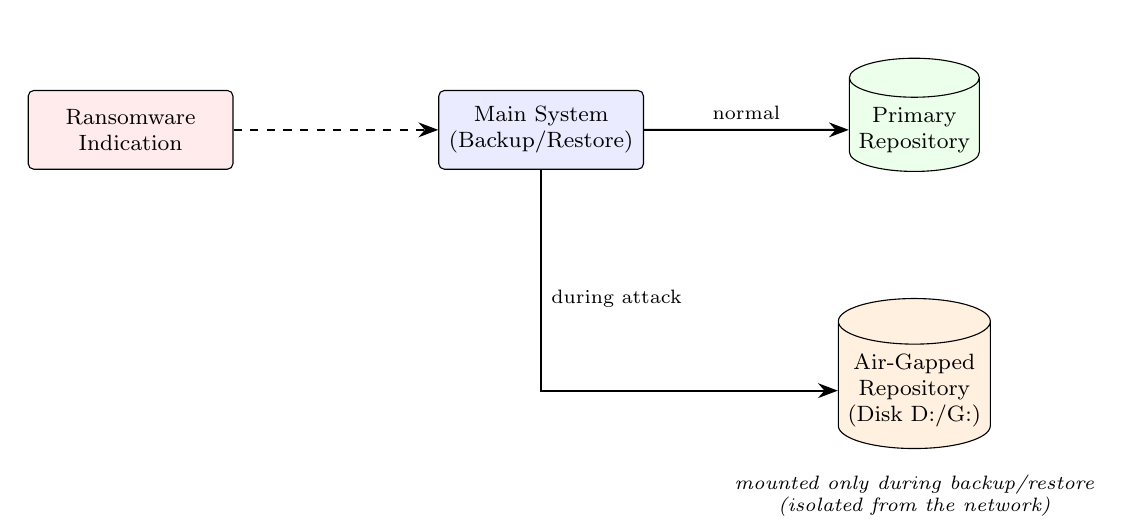
\begin{tikzpicture}[
    font=\footnotesize,
    box/.style={draw, rounded corners=2pt, minimum width=2.6cm, minimum height=1cm, align=center},
    store/.style={draw, cylinder, shape border rotate=90, aspect=0.3, minimum width=1.6cm, minimum height=1.4cm, align=center},
    ar/.style={-{Stealth[length=2.5mm]}, thick},
    ard/.style={-{Stealth[length=2.5mm]}, thick, dashed}
]
\node[box, fill=blue!8] (sys) {Main System\\(Backup/Restore)};
\node[store, right=2.6cm of sys, fill=green!8] (primary) {Primary\\Repository};
\node[store, below=1.6cm of primary, fill=orange!12] (airgap) {Air-Gapped\\Repository\\(Disk D:/G:)};
\node[box, left=2.6cm of sys, fill=red!8] (att) {Ransomware\\Indication};
\draw[ar] (sys) -- node[above]{\scriptsize normal} (primary);
\draw[ard] (att) -- (sys);
\draw[ar] (sys.south) |- node[below right, font=\scriptsize, pos=0.25]{\scriptsize during attack} (airgap.west);
\node[align=center, below=0.2cm of airgap, font=\scriptsize\itshape] {mounted only during backup/restore\\(isolated from the network)};
\end{tikzpicture}%
}
\vspace{.4em}
\caption{VHDX media-based air-gapped backup architecture with network separation}
\label{fig:vhdx}
\end{figure}

Files recovered from the air-gapped medium are compressed-and-encrypted, so the system first decrypts (AES-256) then decompresses, and validates by comparing SHA-256 checksums before (sha\_in) and after (sha\_out) recovery; a file is valid when both match. All files were recovered with status [OK]---43 files restored without errors.

Recovery is measured by RTO (time to recover all 43 files from air-gapped storage after anomaly detection) on AWS EC2 with a $\approx490$~MB dataset (Table~\ref{tab:rto}). Each scenario recovered 43/43 files without error.

\begin{table}[htbp]
\centering
\fontsize{8pt}{10pt}\selectfont
\caption{Measured Recovery Time Objective (RTO) for recovering all 43 files}
\label{tab:rto}
\begin{tabular}{l c c c}
\hline
\textbf{Attack Type} & \textbf{Total Files} & \textbf{Files Recovered} & \textbf{RTO (s)} \\
\hline
Encrypt-and-Hold (CVE-2017-0144)           & 43 & 43 & 4.34 \\
Metadata/Header Corruption (CVE-2018-8453) & 43 & 43 & 5.21 \\
Overwrite-and-Corrupt (CVE-2021-36934)     & 43 & 43 & 5.34 \\
\hline
\end{tabular}
\end{table}

RTO ranges 4.3--5.3~s for the whole test dataset. Because the workflow is deterministic and grows about linearly with volume, RTO extrapolates proportionally for enterprise scale; full-scale validation (files up to 1~GB) is future work.

\subsection{Cross-platform consistency (Windows vs Linux)}
The same experiment ran on AWS EC2 Windows Server 2022 and Ubuntu 22.04. Compression savings are practically identical on both (e.g., Log/TXT with Brotli 89.6\% vs 89.5\%, CSV 81.1\% vs 81.1\%, JPG/XLSX $\approx$0\%), since they depend on data and algorithm rather than OS, and detection/recovery are perfect on both (43/43, FPR/FNR 0\%). Only RTO differs slightly due to hardware, as summarized in Table~\ref{tab:cross_platform}.

\begin{table}[htbp]
\centering
\fontsize{8pt}{10pt}\selectfont
\caption{Cross-platform recovery time (RTO, seconds) by attack type (43 files)}
\label{tab:cross_platform}
\begin{tabular}{l c c}
\hline
\textbf{Attack Type} & \textbf{Windows Server 2022} & \textbf{Ubuntu 22.04} \\
\hline
Encrypt-and-Hold        & 5.50 & 4.34 \\
Metadata Corruption     & 5.20 & 5.21 \\
Overwrite-and-Corrupt   & 5.32 & 5.34 \\
\hline
\end{tabular}
\end{table}

This agreement confirms that adaptive compression, integrity verification, and air-gapped recovery work reliably and reproducibly on both local Windows and cloud Linux/Windows infrastructure, strengthening external validity.

\subsection{False positive and false negative evaluation}
To assess detection reliability, FPR and FNR were measured by comparing legitimate AES-256 backup encryption against simulated ransomware that modifies content and metadata; on detecting abnormal changes the system auto-activated air-gapped recovery and replaced corrupted files from isolated copies (Table~\ref{tab:detection_accuracy}).

\begin{table}[htbp]
\centering
\fontsize{8pt}{10pt}\selectfont
\caption{Detection and recovery accuracy evaluation}
\label{tab:detection_accuracy}
\begin{tabularx}{\textwidth}{@{}X c c c c c@{}}
\hline
\textbf{Scenario} & \textbf{Total Files} & \textbf{Detected as Ransomware} & \textbf{Auto Air-Gapped Restore} & \textbf{Actual Status} & \textbf{Result} \\
\hline
Normal AES-256 backup encryption & 43 & 0 & No & Safe & True Negative \\
Encrypt and Hold attack & 43 & 43 & Yes & Ransomware & True Positive \\
Metadata/Header Corruption & 43 & 43 & Yes & Ransomware & True Positive \\
Overwrite and Corrupt & 43 & 43 & Yes & Ransomware & True Positive \\
\hline
\end{tabularx}
\end{table}

The results yield FPR = 0\% and FNR = 0\%: the system distinguishes legitimate AES-256 backup encryption from unauthorized ransomware modification, and on detecting anomalies auto-restores clean versions from air-gapped backup.

These 0\% values are a logical consequence of hash-integrity detection in a controlled environment, not a claim of perfect real-world detection: any modification deterministically changes the SHA-256 hash, so all simulated corruption is detected, while legitimate encryption is never falsely flagged because its baseline is recorded beforehand. Integrity-based mechanisms detect that a file changed but not the behavior of a process, so they remain vulnerable to sophisticated evasion (FPE, fileless, Living-off-the-Land) not represented in our synthetic dataset. The figures thus validate the mitigation/recovery stage functionally, not detection accuracy in general.

\subsection{Security analysis of the logical air-gap and window of vulnerability}
Unlike a physical air-gap that fully severs the connection, the logical air-gap isolates the backup volume by mounting it only during an active backup/recovery window. This is more affordable and practical but leaves a window of vulnerability: while mounted, the volume is reachable by other host processes, and memory-resident ransomware could wait for a mount event to write a payload. Logical isolation therefore substantially reduces, but does not eliminate, the attack surface versus a continuously connected repository. To narrow this window, we recommend: (i) strict IAM access control so only authorized backup processes may mount and write; (ii) read-only mount during recovery; (iii) immutable/WORM storage (e.g., object lock) so written versions cannot be altered or deleted during retention; and (iv) minimizing mount duration. Together these make the logical air-gap a reasonable balance of cost and resilience, pointing toward a zero-trust backup architecture in future work.

\section{Conclusion}
\label{sec:conclusion}
A cloud-based backup system integrating an air-gapped mechanism with multi-algorithm lossless compression was developed to improve ransomware resilience while optimizing storage. It performs compression, backup, anomaly detection, and automated recovery in one integrated environment. Compression performance depends on data characteristics: Snappy/LZ4 are faster for small-to-medium files, while Brotli/Zstandard achieve the highest ratios on low-entropy text (savings up to 89.5\% for logs and 81.1\% for CSV); already-compressed JPG/XLSX save near zero, matching the lossless limit.

Controlled ransomware simulations (no real malware) on a 43-file synthetic dataset, using CVE-2017-0144, CVE-2018-8453, and CVE-2021-36934 patterns, showed the system preserved integrity and achieved 100\% recovery across all 43 files via the air-gapped mechanism, with the anomaly detector flagging unauthorized modifications while keeping zero false positives on legitimate AES-256 operations. Integrating air-gapped backup with multi-algorithm compression thus significantly enhances both resilience and storage efficiency in cloud backup.

The adaptive mechanism uses rule-based selection for its low overhead, lightweight implementation, and fast decisions---suited to financial cloud systems needing reliability and low-latency operation. Limitations open future directions: validation used a limited synthetic dataset (43 files) via controlled simulation, so generalization to enterprise scale and real ransomware remains to be tested; and detection relies on hash/metadata integrity, not yet handling sophisticated evasion. Promising directions: (i) evolving rule-based selection into machine learning (e.g., \textit{Random Forest}) for larger, heterogeneous data; (ii) testing real ransomware in a safe \textit{sandbox}; (iii) integrating immutable/WORM storage and zero-trust backup; (iv) formal security analysis and stronger \textit{key management}; (v) enterprise-scale evaluation of throughput, CPU/RAM, energy, and cloud cost; and (vi) comparison with \textit{incremental backup} and \textit{deduplication}. These would further strengthen the credibility, resilience, and practical feasibility of the ransomware-resilient backup system.

\section*{ACKNOWLEDGEMENTS}
\label{sec:ack}
The authors thank Politeknik Elektronika Negeri Surabaya for the research facilities and PT Equnix Business Solution for the collaboration and insight into enterprise backup practices that informed the design of the synthetic dataset.

\section*{FUNDING INFORMATION}
\label{sec:funding}
This research was funded by the Ministry of Higher Education, Science, and Technology of the Republic of Indonesia (Kementerian Pendidikan Tinggi, Sains, dan Teknologi Republik Indonesia) in 2026.

\section*{AUTHOR CONTRIBUTIONS STATEMENT}
\label{sec:credit}
This study employs the Contributor Roles Taxonomy (CRediT) to acknowledge individual author contributions, mitigate authorship conflicts, and enhance collaboration.

\begin{table}[htbp]
	\centering
	\selectfont
	\begin{tabular}{lcccccccccccccc}
		\hline
		\textbf{Name of Author} & \cellcolor[HTML]{D8F0F8}\textbf{C} & \cellcolor[HTML]{D8F0F8}\textbf{M} & \textbf{So} & \textbf{Va} & \cellcolor[HTML]{D8F0F8}\textbf{Fo} & \cellcolor[HTML]{D8F0F8}\textbf{I} & \textbf{R} & \textbf{D} & \cellcolor[HTML]{FDE9D9}\textbf{O} & \cellcolor[HTML]{FDE9D9}\textbf{E} & \textbf{Vi} & \textbf{Su} & \textbf{P} & \textbf{Fu} \\
		\hline
		Hero Yudo Martono & \cellcolor[HTML]{D8F0F8}\checkmark & \cellcolor[HTML]{D8F0F8}\checkmark & \checkmark & \checkmark & \cellcolor[HTML]{D8F0F8}\checkmark & \cellcolor[HTML]{D8F0F8}\checkmark &  & \checkmark & \cellcolor[HTML]{FDE9D9}\checkmark & \cellcolor[HTML]{FDE9D9}\checkmark &  & \checkmark & \checkmark & \checkmark \\
		Nafisah Rahmadani H. & \cellcolor[HTML]{D8F0F8} & \cellcolor[HTML]{D8F0F8}\checkmark & \checkmark &  & \cellcolor[HTML]{D8F0F8}\checkmark & \cellcolor[HTML]{D8F0F8}\checkmark & \checkmark & \checkmark & \cellcolor[HTML]{FDE9D9}\checkmark & \cellcolor[HTML]{FDE9D9} & \checkmark &  &  &  \\
		Iwan Syarif & \cellcolor[HTML]{D8F0F8}\checkmark & \cellcolor[HTML]{D8F0F8}\checkmark &  & \checkmark & \cellcolor[HTML]{D8F0F8} & \cellcolor[HTML]{D8F0F8} &  &  & \cellcolor[HTML]{FDE9D9} & \cellcolor[HTML]{FDE9D9}\checkmark &  & \checkmark &  &  \\
		Ferry Astika Saputra & \cellcolor[HTML]{D8F0F8}\checkmark & \cellcolor[HTML]{D8F0F8}\checkmark &  & \checkmark & \cellcolor[HTML]{D8F0F8} & \cellcolor[HTML]{D8F0F8} &  &  & \cellcolor[HTML]{FDE9D9} & \cellcolor[HTML]{FDE9D9}\checkmark &  & \checkmark &  &  \\
		\hline
		\multicolumn{15}{c}{
			\begin{tabular}{llllll}
				&&&&&\\
				C &: 	\textbf{C}\fontsize{8}{10}\selectfont onceptualization \quad\quad\quad\quad\quad\quad& I &: 	\textbf{I}\fontsize{8}{10}\selectfont nvestigation & Vi&: 	\textbf{Vi}\fontsize{8}{10}\selectfont sualization  \\
				M &: 	\textbf{M}\fontsize{8}{10}\selectfont ethodology & R &: 	\textbf{R}\fontsize{8}{10}\selectfont esources & Su&: 	\textbf{Su}\fontsize{8}{10}\selectfont pervision  \\
				So&: 	\textbf{So}\fontsize{8}{10}\selectfont ftware & D &:	\textbf{D}\fontsize{8}{10}\selectfont ata Curation & P &: 	\textbf{P}\fontsize{8}{10}\selectfont roject Administration  \\
				Va&: 	\textbf{Va}\fontsize{8}{10}\selectfont lidation & O &:	\fontsize{8}{10}\selectfont Writing - \fontsize{10}{12}\selectfont \textbf{O}\fontsize{8}{10}\selectfont riginal Draft & Fu&: 	\textbf{Fu}\fontsize{8}{10}\selectfont nding Acquisition \\
				Fo&: 	\textbf{Fo}\fontsize{8}{10}\selectfont rmal Analysis & E &:	\fontsize{8}{10}\selectfont Writing - Review \& \fontsize{10}{12}\selectfont\textbf{E}\fontsize{8}{10}\selectfont diting \quad\quad\quad\quad\quad\quad&  \\
			\end{tabular}
		}
	\end{tabular}
\end{table}

\section*{CONFLICT OF INTEREST STATEMENT}
\label{sec:coi}
The authors declare that there is no conflict of interest regarding the publication of this paper.

\section*{DATA AVAILABILITY}
\label{sec:data}
Datasets used in this study were synthetically generated based on operational data characteristics and backup structures adapted from PT Equnix Business Solution environments. No real financial or confidential production data were used in this study.

\begin{thebibliography}{99}
\footnotesize
\itemsep 0pt

\bibitem{1} A. A. Majmuah, ``Survey on technique to prevent ransomware attack,'' \textsl{Bulletin of Informatics and Data Science}, vol. 1, no. 2, 2021.
\bibitem{2} K. Begovi\'c, A. Al-Ali, and Q. Malluhi, ``Cryptographic ransomware encryption detection: survey,'' \textsl{Computers \& Security}, vol. 132, art. 103349, 2023, doi: 10.1016/j.cose.2023.103349.
\bibitem{6} G. Lu, Y. Liu, Y. Chen, C. Zhang, Y. Gao, and G. Zhong, ``A comprehensive detection approach of WannaCry: principles, rules and experiments,'' in \textsl{Proc. Int. Conf. Cyber-Enabled Distributed Computing and Knowledge Discovery (CyberC)}, 2020, pp. 41--49.
\bibitem{7} I. Athauda and H. Herath, ``Windows elevation of privilege serious SAM vulnerability (CVE-2021-36934),'' \textsl{Journal of Cybersecurity and Digital Forensics}, 2022.
\bibitem{8} H. Oz, A. Aris, A. Levi, and A. S. Uluagac, ``A survey on ransomware: evolution, taxonomy, and defense solutions,'' \textsl{ACM Computing Surveys}, vol. 54, no. 11s, art. 238, 2022, doi: 10.1145/3514229.
\bibitem{9} Z. A. Syed and T. R. Soomro, ``Compression algorithms: Brotli, Gzip and Zopfli perspective,'' \textsl{International Journal of Computer Science and Network Security}, 2021.
\bibitem{10} F. A. Abdulazeez, I. T. Ahmed, and B. T. Hammad, ``Performance comparison of compression algorithms for large-scale log systems,'' \textsl{Journal of Computer \& Electrical Engineering Sciences}, 2024.
\bibitem{13} M. Sahu and J. Panda, ``Performance evaluation of efficient hybrid compression methods for Devanagari-encoded Hindi text using lossless algorithms,'' \textsl{arXiv preprint arXiv:2504.20747}, 2025, doi: 10.48550/arXiv.2504.20747.
\bibitem{14} H. Zhang et al., ``Optimized Snappy compression with enhanced encoding strategies,'' \textsl{Electronics}, 2024.
\bibitem{19} Sophos, ``The state of ransomware in financial services 2024,'' Sophos Ltd., 2024. [Online]. Available: https://www.sophos.com
\bibitem{20} R. Pal, M. Shaikh, J. Sagvekar, and P. Tiwari, ``Data resilience: secure emergency backup on cloud,'' \textsl{International Journal of Advanced Research in Science, Communication and Technology}, vol. 4, no. 7, 2024.
\bibitem{21} NIST, ``Security guidelines for storage infrastructure (SP 800-209),'' National Institute of Standards and Technology, 2024. [Online]. Available: https://nvlpubs.nist.gov
\bibitem{22} A. Nasif, Z. A. Othman, and N. S. Sani, ``The deep learning solutions on lossless compression methods for alleviating data load on IoT nodes in smart cities,'' \textsl{Sensors}, vol. 21, no. 12, p. 4223, 2021.
\bibitem{23} T. McIntosh, T. Susnjak, T. Liu, D. Xu, P. Watters, D. Liu, Y. Hao, A. Ng, and M. Halgamuge, ``Ransomware reloaded: re-examining its trend, research and mitigation in the era of data exfiltration,'' \textsl{ACM Computing Surveys}, vol. 57, no. 1, art. 18, pp. 1--40, 2024, doi: 10.1145/3691340.
\bibitem{26} C. Beaman, A. Barkworth, T. D. Akande, S. Hakak, and M. K. Khan, ``Ransomware: recent advances, analysis, challenges and future research directions,'' \textsl{Computers \& Security}, vol. 111, p. 102490, 2021, doi: 10.1016/j.cose.2021.102490.
\bibitem{27} M. Dawood et al., ``Cyberattacks and security of cloud computing: a complete guideline,'' \textsl{Symmetry}, vol. 15, no. 11, p. 1981, 2023.
\bibitem{29} P. Novak et al., ``Multistage malware detection method for backup systems,'' \textsl{Technologies}, vol. 12, no. 2, p. 23, 2024.
\bibitem{30} Kritika, ``A comprehensive literature review on ransomware detection using deep learning,'' \textsl{Cyber Security and Applications}, vol. 3, p. 100078, 2025, doi: 10.1016/j.csa.2024.100078.
\bibitem{31} N. Ebrahimi Majd and T. Mazumdar, ``Ransomware classification using machine learning,'' in \textsl{Proc. 32nd Int. Conf. Advanced Information Networking and Applications (AINA)}, IEEE, 2023.
\bibitem{32} S. Enomoto, H. Kuzuno, H. Yamada, Y. Shiraishi, and M. Morii, ``Early mitigation of CPU-optimized ransomware using monitoring encryption instructions,'' \textsl{International Journal of Information Security}, vol. 23, pp. 3393--3413, 2024, doi: 10.1007/s10207-024-00892-2.
\bibitem{36} K. Mazel, A. P. Maharani, C. Averill, and R. Patel, ``Comparative study of data compression algorithms: Zstandard, zlib and LZ4,'' in \textsl{Proc. Int. Conf. on Computing and Informatics}, Lecture Notes in Networks and Systems, Springer, 2024, doi: 10.1007/978-3-031-72284-4\_24.
\bibitem{37} C. Jaranilla and J. Choi, ``Requirements and trade-offs of compression techniques in key--value stores: a survey,'' \textsl{Electronics}, vol. 12, no. 20, art. 4280, 2023, doi: 10.3390/electronics12204280.
\bibitem{38} P. G. Shynu, R. K. Nadesh, V. G. Menon, P. Venu, M. Abbasi, and M. R. Khosravi, ``A secure data deduplication system for integrated cloud-edge networks,'' \textsl{Journal of Cloud Computing}, vol. 9, art. 61, 2020, doi: 10.1186/s13677-020-00214-6.
\bibitem{39} K. R. Vaidya, D. Kannur Munirathnam, and P. Seeling, ``Lossless compression for the model context protocol: energy consumption, latency, and bandwidth trade-offs,'' \textsl{Sensors}, vol. 26, no. 14, art. 4582, 2026, doi: 10.3390/s26144582.
\bibitem{41} G. Nagar, ``The evolution of ransomware: tactics, techniques, and mitigation strategies,'' \textsl{SSRN Electronic Journal}, 2024, doi: 10.2139/ssrn.4881213.
\bibitem{42} A. Kapoor, A. Gupta, R. Gupta, S. Tanwar, G. Sharma, and I. E. Davidson, ``Ransomware detection, avoidance, and mitigation scheme: a review and future directions,'' \textsl{Sustainability}, vol. 14, no. 1, p. 8, 2022, doi: 10.3390/su14010008.
\bibitem{43} J. Lee, J. Kim, H. Jeong, and K. Lee, ``A machine learning-based ransomware detection method for attackers' neutralization techniques using format-preserving encryption,'' \textsl{Sensors}, vol. 25, no. 8, p. 2406, 2025, doi: 10.3390/s25082406.
\bibitem{44} J. Thomas and G. Galligher, ``Improving backup system evaluations in information security risk assessments to combat ransomware,'' \textsl{Computer and Information Science}, vol. 11, no. 1, pp. 25--38, 2018, doi: 10.5539/cis.v11n1p25.
\bibitem{45} B. Bahl and R. Endicott, ``Know thy ransomware response: a detailed framework for devising effective ransomware response strategies,'' \textsl{Digital Threats: Research and Practice}, vol. 4, no. 4, pp. 1--19, 2020, doi: 10.1145/3560022.
\bibitem{46} P. Yan and T. T. Khoei, ``Securing the Internet of Things: a comprehensive review of ransomware attacks, detection, countermeasures, and future prospects,'' \textsl{Franklin Open}, vol. 11, art. 102056, 2025, doi: 10.1016/j.fraope.2025.102056.

\end{thebibliography}

\section*{BIOGRAPHIES OF AUTHORS}
\label{sec:biographies}
% IJECE TEMPLATE REQUIREMENT (profile icons): each biography must end with the
% author's linked profile icons -- ORCID, Scopus, Web of Science (Publons), and
% Google Scholar -- and no icon may be deleted. The ORCID iD placeholder
% \orcidlink{0000-0000-0000-0000} is included for each author below; replace it
% with the real ORCID iD. When compiling in the official IJECE Overleaf project,
% add the Scopus / WoS / Scholar icons immediately after \orcidlink using the
% template's built-in icon macros and link each to the author's profile.

\noindent
\begin{tabularx}{\textwidth}{@{}m{2.5cm}@{\hspace{0.4cm}}X@{}}
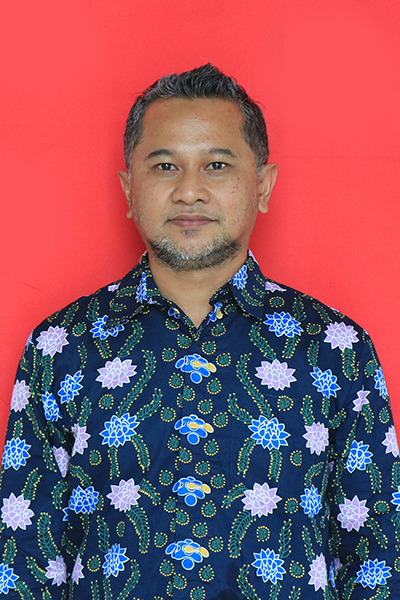
\includegraphics[width=2.5cm,height=3.2cm,keepaspectratio]{figures/hero_yudo.jpg} &
\textbf{Hero Yudo Martono} received his bachelor's degree in Computer Science (Electrical Engineering) from ITS, Indonesia. He then pursued a master's degree in Informatics Engineering from ITB, Indonesia. His research interests include cybersecurity, artificial intelligence, and cloud computing. He can be contacted at email: hero@pens.ac.id. \orcidlink{0000-0000-0000-0000} \\
\end{tabularx}

\vspace{.7em}
\noindent
\begin{tabularx}{\textwidth}{@{}m{2.5cm}@{\hspace{0.4cm}}X@{}}
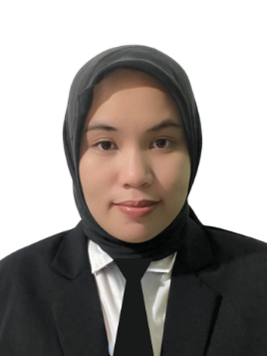
\includegraphics[width=2.5cm,height=3.2cm,keepaspectratio]{figures/nafisah.png} &
\textbf{Nafisah Rahmadani Harahap} is currently pursuing the Bachelor of Applied Engineering (D4) degree in Informatics Engineering at Politeknik Elektronika Negeri Surabaya (PENS), Indonesia. She is also working as an ERP Project Manager, focusing on enterprise resource planning implementation, business process optimization, project coordination, and digital transformation initiatives. Her research interests include cybersecurity, information systems, artificial intelligence, cloud computing, and enterprise software solutions. She can be contacted at email: nafisah@it.student.pens.ac.id. \orcidlink{0000-0000-0000-0000} \\
\end{tabularx}

\vspace{.7em}
\noindent
\begin{tabularx}{\textwidth}{@{}m{2.5cm}@{\hspace{0.4cm}}X@{}}
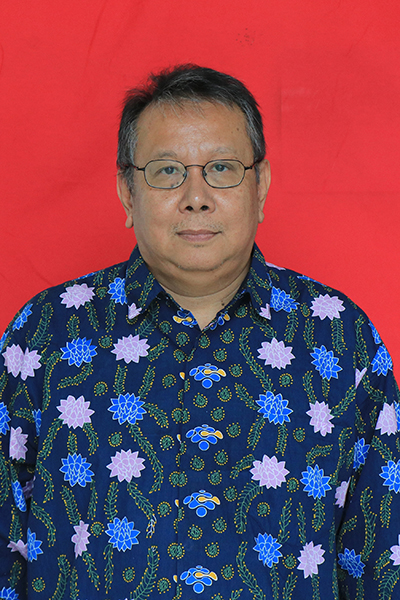
\includegraphics[width=2.5cm,height=3.2cm,keepaspectratio]{figures/iwan_syarif.jpg} &
\textbf{Iwan Syarif} is a professor (Ph.D.) and lecturer at the Department of Informatics Engineering, Politeknik Elektronika Negeri Surabaya (PENS), Indonesia. His research focuses on cybersecurity. He can be contacted at email: iwanarif@pens.ac.id. \orcidlink{0000-0000-0000-0000} \\
\end{tabularx}

\vspace{.7em}
\noindent
\begin{tabularx}{\textwidth}{@{}m{2.5cm}@{\hspace{0.4cm}}X@{}}
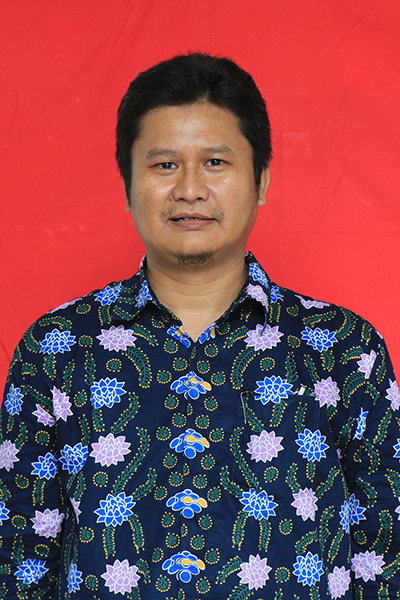
\includegraphics[width=2.5cm,height=3.2cm,keepaspectratio]{figures/ferry_astika.jpg} &
\textbf{Ferry Astika Saputra} received his doctoral (Ph.D.) degree from Universitas Indonesia and is a lecturer at the Department of Informatics Engineering, Politeknik Elektronika Negeri Surabaya (PENS), Indonesia. His research focuses on cybersecurity. He can be contacted at email: ferryas@pens.ac.id. \orcidlink{0000-0000-0000-0000} \\
\end{tabularx}

\end{document}
